\documentclass{article}
\title{Getting Started with XShaderCompiler}
\author{Lukas Hermanns}
\date{\today}

\usepackage{listings}
\usepackage{color}
\usepackage{pxfonts}
\usepackage{geometry}
\usepackage[T1]{fontenc}
\usepackage{xspace}
\usepackage{hyperref}
\usepackage{graphicx}
\usepackage{float}
\usepackage{pdfpages}

\geometry{
	a4paper,
	left=15mm,
	right=15mm,
	top=20mm,
	bottom=20mm
}

\begin{document}

\definecolor{brightBlueColor}{rgb}{0.5, 0.5, 1.0}
\definecolor{darkBlueColor}{rgb}{0.0, 0.0, 0.5}

\def\XSC{\textcolor{darkBlueColor}{XShaderCompiler}\xspace}

\lstset{
	language = C++,
	basicstyle = \footnotesize\ttfamily,
	commentstyle = \itshape\color{brightBlueColor},
	keywordstyle = \bfseries\color{darkBlueColor},
	stringstyle = \color{red},
	frame = single,
	tabsize = 4,
	showstringspaces = false,
	numbers = none
}

\lstdefinelanguage{hlslLanguage}
{
	morekeywords = {
		float2, float3, float4, float4x4 % ...
	},
}

\lstdefinelanguage{glslLanguage}
{
	morekeywords = {
		vec2, vec3, vec4, mat4 % ...
	},
}

\maketitle

%\begin{figure}[ht]
%	\centering
%	\includegraphics[width=0.5\textwidth]{../XShaderCompiler_Logo.pdf}
%\end{figure}

\newpage


%----------------------------------------------------------------------------------------
%	CONTENTS
%----------------------------------------------------------------------------------------

\tableofcontents

\newpage


%----------------------------------------------------------------------------------------
%	INTRRODUCTION
%----------------------------------------------------------------------------------------

\section{Introduction}

\XSC (``Cross Shader Compiler'') is a cross-compiler (also called trans-compiler),
which translates HLSL code (DirectX High Level Shading Language,
see \href{https://msdn.microsoft.com/en-us/library/windows/desktop/bb509561(v=vs.85).aspx}{msdn.microsoft.com}) 
of Shader Model 3, 4, and 5 into GLSL code (OpenGL Shading Language,
see \href{https://www.opengl.org/wiki/OpenGL_Shading_Language}{www.opengl.org}).


%----------------------------------------------------------------------------------------
%	PROGRESS
%----------------------------------------------------------------------------------------

\newpage
\section{Progress}

This project is still in its early steps. This document is written for \XSC \textbf{Version 0.02 Alpha}.

\subsection{ToDo List}
\begin{itemize}
	\item \textbf{Geometry Shader Semantic}
	\item \textbf{Tessellation Shader Semantic}
\end{itemize}


%----------------------------------------------------------------------------------------
%	OFFLINE COMPILER
%----------------------------------------------------------------------------------------

\newpage
\section{Offline Compiler}

The offline compiler (named \texttt{xsc}) can be used to cross-compile your shaders without building any custom application.
It has similar commands like other common compilers (such as GCC), e.g. \texttt{-O} to enable optimization.
To show the description of all commands, type simply \texttt{xsc} or \texttt{xsc --help} into a terminal or command line.

\subsection{Commands}

Here is an overview of the most important commands:
\begin{itemize}
	\item[] \textbf{\texttt{-T, ----target \textit{TARGET}}} \\
	Sets the shader target specified by \texttt{\textit{TARGET}}.
	Valid values for \texttt{\textit{TARGET}} are:
	\begin{itemize}
		\item[] \textbf{\texttt{vert}} (for \textbf{Vert}ex Shader)
		\item[] \textbf{\texttt{tesc}} (for \textbf{Tes}sellation \textbf{C}ontrol Shader, also called Hull Shader)
		\item[] \textbf{\texttt{tese}} (for \textbf{Tes}sellation \textbf{E}valuation Shader, also called Domain Shader)
		\item[] \textbf{\texttt{geom}} (for \textbf{Geom}etry Shader)
		\item[] \textbf{\texttt{frag}} (for \textbf{Frag}ment Shader, also called Pixel Shader)
		\item[] \textbf{\texttt{comp}} (for \textbf{Comp}ute Shader)
	\end{itemize}
	
	\item[] \textbf{\texttt{-E, ----entry \textit{ENTRY}}} \\
	Sets the shader entry point (i.e. main function) specified by \texttt{\textit{ENTRY}}.
	
	\item[] \textbf{\texttt{-I, ----include-path \textit{PATH}}} \\
	Adds the file path, specified by \texttt{\textit{PATH}}, to the include search paths.
	
	\item[] \textbf{\texttt{-o, ----output \textit{FILE}}} \\
	Sets the filename of the output file specified by \texttt{\textit{FILE}}.
	The default value is ``\texttt{\textit{FILE}.\textit{ENTRY}.\textit{TARGET}}'',
	where \texttt{\textit{FILE}} is the filename of the input shader file, \texttt{\textit{ENTRY}} is the shader entry point,
	and \texttt{\textit{TARGET}} is the shader output target. The asterisk character `*' can be included to
	re-use the default value, e.g. ``\texttt{OutputFolder/*}'' will result into
	``\texttt{OutputFolder/\textit{FILE}.\textit{ENTRY}.\textit{TARGET}}''
	
	\item[] \textbf{\texttt{-Vin, ----version-in \textit{VERSION}}} \\
	Sets the input shader version specified by \texttt{\textit{VERSION}}.
	Valid values for \texttt{\textit{VERSION}} are:
	\begin{itemize}
		\item[] \textbf{\texttt{HLSL3}} (for HLSL Shader Model 3)
		\item[] \textbf{\texttt{HLSL4}} (for HLSL Shader Model 4)
		\item[] \textbf{\texttt{HLSL5}} (for HLSL Shader Model 5) \textit{default value}
	\end{itemize}
	
	\item[] \textbf{\texttt{-Vout, ----version-out \textit{VERSION}}} \\
	Sets the output shader version specified by \texttt{\textit{VERSION}}.
	Valid values for \texttt{\textit{VERSION}} are:
	\begin{itemize}
		\item[] \textbf{\texttt{GLSL}} (for automatic deduction of the minimal required GLSL version) \textit{default value}
		\item[] \textbf{\texttt{GLSL110}} (for GLSL 1.10) \textit{not supported yet}
		\item[] \textbf{\texttt{GLSL120}} (for GLSL 1.20) \textit{not supported yet}
		\item[] \textbf{\texttt{GLSL130}} (for GLSL 1.30)
		\item[] \textbf{\texttt{GLSL140}} (for GLSL 1.40)
		\item[] \textbf{\texttt{GLSL150}} (for GLSL 1.50)
		\item[] \textbf{\texttt{GLSL330}} (for GLSL 3.30)
		\item[] \textbf{\texttt{GLSL400}} (for GLSL 4.00)
		\item[] \textbf{\texttt{GLSL410}} (for GLSL 4.10)
		\item[] \textbf{\texttt{GLSL420}} (for GLSL 4.20)
		\item[] \textbf{\texttt{GLSL430}} (for GLSL 4.30)
		\item[] \textbf{\texttt{GLSL440}} (for GLSL 4.40)
		\item[] \textbf{\texttt{GLSL450}} (for GLSL 4.50)
	\end{itemize}
	
\end{itemize}

\subsection{Error Output}

\XSC has an extensive report handler for meaningful output messages.
It even has a line marker, to show the source line where the error (or warning) occured.
This can be very handy because the line marker acts like a picture, and a picture is worth a thousand words ;-)
Take a look at the following example, where the slot register `\texttt{b0}' uses a target specific profile
(here `\texttt{vs}' for the Vertex Shader):
\begin{figure}[H]
	\centering
	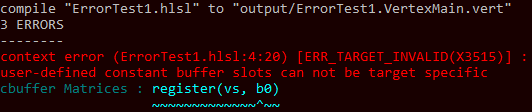
\includegraphics{images/error_output1}
	\caption{Error output example of \XSC.}
	\label{fig:error_output1}
\end{figure}
There are a couple of things displayed in this error message, which we will go thorugh step by step:
\begin{enumerate}
	\item \textbf{\texttt{context error}} \\
	This indicates that the error occured during the context analysis. The compilation phases are:
	\emph{pre-processing}, \emph{syntax parsing}, \emph{context analysis},
	\emph{post-processing} (optimization and conversion for the target language), and \emph{code generation}.
	
	\item \textbf{\texttt{(ErrorTest1.hlsl:4:20)}} \\
	The part in the brackets shows the source position in the input code.
	Here the filename is ``\texttt{ErrorTest1.hlsl}'', the row is 4, and the column is 20.
	
	\item \textbf{\texttt{[ERR\_TARGET\_INVALID(X3515)]}} \\
	This part does only appear in a couple of types of errors. It shows the error code, which is commonly only
	displayed as the number within the brackets, but the \XSC also shows the identifier.
	
	\item \textbf{\texttt{user-defined constant buffer slots can not be target specific}} \\
	This is the actual error message, which describes the compilation conflict.
\end{enumerate}
Here is another example how the line marker can show very intuitively what the problem is:
\begin{figure}[H]
	\centering
	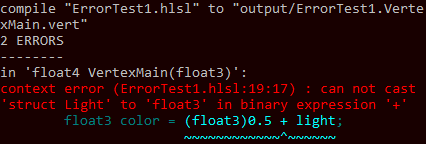
\includegraphics{images/error_output2}
	\caption{Error output example of \XSC.}
	\label{fig:error_output2}
\end{figure}
Here the variable \texttt{light}, which is from type \texttt{struct Light}, can not be casted
to a \texttt{float3} type within a concatenation like the `+' operator.


%----------------------------------------------------------------------------------------
%	API OVERVIEW
%----------------------------------------------------------------------------------------

%\newpage
%\section{API Overview}





%----------------------------------------------------------------------------------------
%	APPENDIX
%----------------------------------------------------------------------------------------

%\newpage

%\section{Appendix}

%Foo bar ...


\end{document}
